\documentclass{beamer}

\usepackage[utf8]{inputenc}
\usepackage[spanish]{babel}

\usetheme{boxes}
\usecolortheme{beaver}
\setbeamercolor{alerted text}{fg = blue}

%code
\usepackage{listings}

\title[]{Preprocesamiento de Imágenes Mamográficas}
\author{Omar Trinidad Gutiérrez Méndez\\Juana Canul Reich}
\institute{División Académica de Informática y Sistemas\\Semana de Divulgación y Video Científico}
\date{Septiembre de 2013}

\beamertemplateshadingbackground{gray!40}{white!2}

\begin{document}

\begin{frame}{}
  \transdissolve
  \titlepage
  \begin{figure}
    \centering
     
\includegraphics[height=1.66cm]{images/logo-dais.png}
  \end{figure}
\end{frame}


\section{Introducción}
\subsection{Cáncer de mama}
\begin{frame}{Cáncer de mama}
\transdissolve
   \pause
   %\setbeamercovered{transparent}
   \begin{itemize}
        \item<2-> \alt<2>{\color{blue}El cáncer de mama es un grave problema de salud pública}
                         {\color{red!30}El cáncer de mama es un grave problema de salud pública}
        \item<2-> \alt<3>{\color{blue}El estudio de mamografías es la mejor forma de detectar oportunamente este padecimiento}
                         {\color{red!30}El estudio de mamografías es la mejor forma de detectar oportunamente este padecimiento}
        \item<2-> \alt<4>{\color{blue}Existe un margen de error en la opinión de los radiólogos}
                         {\color{red!30}Existe un margen de error en la opinión de los radiólogos}
        \item<2-> \alt<5>{\color{blue}Es posible incrementar los diagnósticos exitosos al mejorar la calidad de la imagen}
                         {\color{red!30}Es posible incrementar los diagnósticos exitosos al mejorar la calidad de la imagen}
   \end{itemize}
\end{frame}

\subsection{Preprocesamiento}
\begin{frame}{Preprocesamiento}
\transdissolve
   \pause
   %\setbeamercovered{transparent}
   \begin{itemize}
        \item<2-> \alt<2>{\color{blue}El preprocesamiento es la fase previa al procesamiento de imágenes \textit{per se}}
                         {\color{red!30}El preprocesamiento es la fase previa al procesamiento de imágenes \textit{per se}}
        \item<2-> \alt<3>{\color{blue}El preprocesamiento es útil para:}
                         {\color{red!30}El preprocesamiento es útil para:}
                         \begin{itemize}
                            \item<2-> \alt<4>{\color{blue}Mejorar la calidad de la imagen al ojo humano}
                                             {\color{red!30}Mejorar la calidad de la imagen al ojo humano}
                            \item<2-> \alt<5>{\color{blue}Preparar la imagen para ser usada en etapas posteriores}
                                             {\color{red!30}Preparar la imagen para ser usada en etapas posteriores}
                         \end{itemize}
   \end{itemize}
\end{frame}

\subsection{Mamogramas}
\begin{frame}{Mamogramas}
\transdissolve
   \pause
   %\setbeamercovered{transparent}
   \begin{itemize}
        \item<2-> \alt<2>{\color{blue}Los mamogramas o mamografías son radiografías de baja intensidad}
                         {\color{red!30}Los mamogramas o mamografías son radiografías de baja intensidad}
        \item<2-> \alt<3>{\color{blue}No son imágenes convencionales}
                         {\color{red!30}No son imágenes convencionales}
        \item<2-> \alt<4>{\color{blue}DICOM (Digital Imaging and COmmunications in Medicine) es el estándar de las imágenes médicas}
                         {\color{red!30}DICOM (Digital Imaging and COmmunications in Medicine) es el estándar de las imágenes médicas}
   \end{itemize}
\end{frame}

\section{Desarrollo}
\subsection{Materiales y métodos}
\begin{frame}{Materiales y métodos}
\transdissolve
  \pause
  \begin{itemize}[<+-| alert@+>]
    \item El Hospital Juan Graham Casasús dió acceso a un banco de mamogramas \textit{crudos}
    \item Se aplicó un enfoque híbrido consistente en los siguientes métodos:
    \begin{itemize}[<+-| alert@+>]
        \item Reducción del área de trabajo
        \item Conversión de bits
        \item Eliminación de ruido
        \item Mejora de contraste
    \end{itemize}
    \item La implementación se realizó con el lenguaje de programación Matlab
    \item También se utilizó Python para ejecutar tareas de \textit{scripting}
  \end{itemize}
\end{frame}

\subsection{Reducción del área de trabajo}
\begin{frame}{Reducción del área de trabajo}
\transdissolve
  \pause
  \begin{figure}
    \centering
     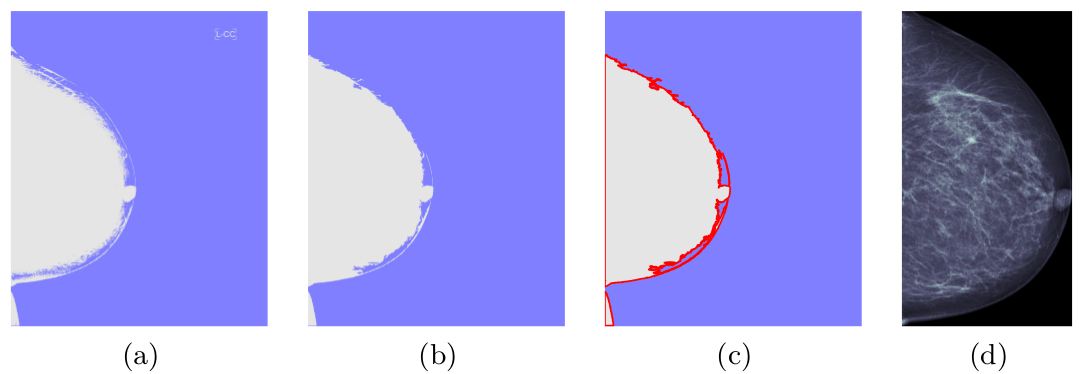
\includegraphics[height=3.66cm]{images/one.png}
  \end{figure}
  \pause
  \begin{itemize}[<+-| alert@+>]
    \item Las mamografías son imágenes de \textit{gran} resolución
    \item En esta etapa se elimina la región oscura de la imagen
    \item Los pasos para reducir el área de trabajo son:
    \begin{itemize}[<+-| alert@+>]
        \item Binarización
        \item Eliminación de etiquetas
        \item Dibujar los bordes
        \item Corte
    \end{itemize}
  \end{itemize}
\end{frame}

\subsection{Conversión de la profundidad de bits}
\begin{frame}{Conversión de la profundidad de bits}
\transdissolve
  \pause
  \begin{figure}
    \centering
     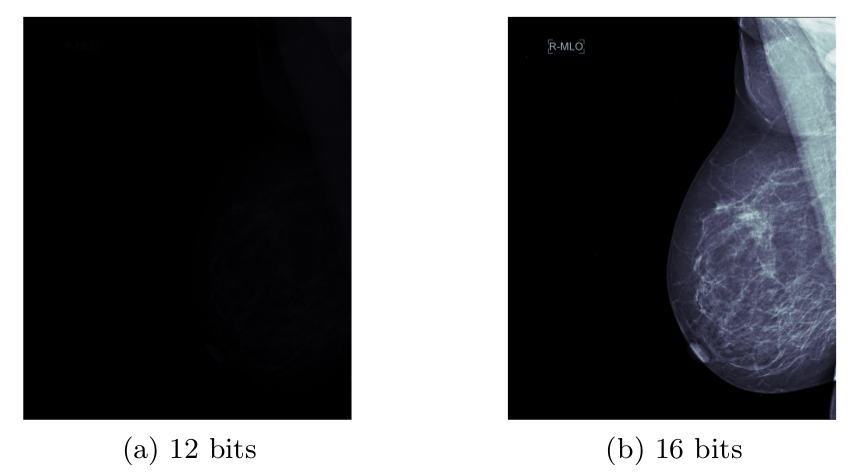
\includegraphics[height=3.66cm]{images/two.png}
  \end{figure}
  \pause
  \begin{itemize}[<+-| alert@+>]
    \item La profundidad de una mamografía es por lo general 12 bits
    \item Matlab está configurado para visualizar las imágenes a 8 ó 16 bits
    \item Al visualizar una mamografía de 12 bits como una imagen de 16 bits, esta luce oscura
  \end{itemize}
\end{frame}

\subsection{Eliminación de ruido}
\begin{frame}{Eliminación de ruido}
\transdissolve
  \pause
  \begin{figure}
    \centering
     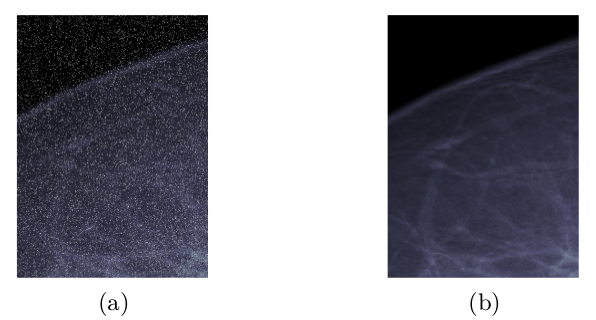
\includegraphics[height=3.66cm]{images/three.png}
  \end{figure}
  \pause
  \begin{itemize}[<+-| alert@+>]
    \item En el proceso de adquisición de los datos es posible obtener algún tipo de contaminación, conocida como ruido
    \item Un ruido común en las imágenes mamográficas es conocido como ruido impulsivo, o ruido de \textit{sal y pimienta}
    \item Se aplicó el Filtro Adaptativo de la Mediana para eliminar el ruido
  \end{itemize}
\end{frame}

\subsection{Mejora de contraste}
\begin{frame}{Mejora de contraste}
\transdissolve
  \pause
  \begin{figure}
    \centering
     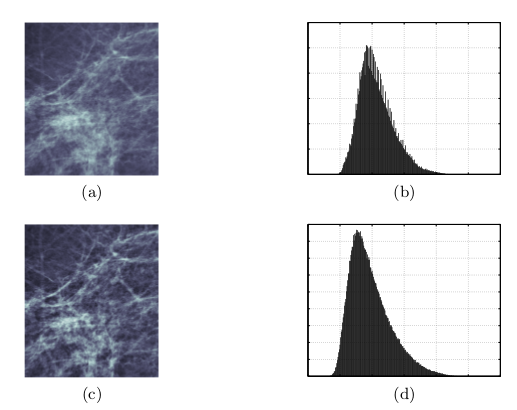
\includegraphics[height=3.66cm]{images/four.png}
  \end{figure}
  \pause
  \begin{itemize}[<+-| alert@+>]
    \item Se utilizó el algoritmo CLAHE (Contrast-Limited Adaptive Histogram Equalization)
    \item Con la ecualización de histogramas se distribuyen mejor los niveles de grises en la imagen
  \end{itemize}
\end{frame}

\section{Conclusiones}
\begin{frame}{Conclusiones}
\transdissolve
  \pause
  \begin{itemize}[<+-| alert@+ >]
    \item Se está construyendo un banco de datos de mamogramas preprocesados
    \item El material será de dominio público
    \item El código fuente empleado es \textit{open source} y puede encontrarse en {\small \url{https://github.com/omartrinidad/preprocessing}}
  \end{itemize}
\end{frame}
\end{document}
